%label:"art:Tropicalchowgroupsii"
%type:"article"
%name:"TropicalChowGroupsII"
%caption:""
%parent:""


The goal of this note is to 
\begin{enumerate}
    \item Define tropical rational equivalence (this works in general, not just in $\RR^n$)
    \item Study Chow group of $\RR^n$
\end{enumerate}
%label:"def:TropicalPolyhedralComplex"
%type:"definition"
%name:"tropical polyhedral complex"
%caption:""
%parent:"art_TropicalChowGroupsII"


    A tropical polyhedral complex is a collection of facets satisfying some balencing conditions. 


%label:"def:EquivalenceOfTropicalPolyhedralComplexes"
%type:"definition"
%name:"equivalence of tropical polyhedral complexes"
%caption:""
%parent:"art_TropicalChowGroupsII"


    A cycle is defined to be an equivalence class of tropical polyhedral complex under the relation of refinement.


%label:"def:TropicalCartierDivisor"
%type:"definition"
%name:"tropical Cartier divisor"
%caption:""
%parent:"art_TropicalChowGroupsII"


    A tropical Carier divisor is an element $\phi\in \mathcal K^*_Q/\mathcal O_Q$.


Recall that $\mathcal K^*_X$ is the ring of tropical rational function \cref{def:TropicalRationalfunction}.
To each tropical Cartier divisor we can construct an associated Weil divisor: take the graph of $\phi$, which is a polyhedral complex; extend this to a balanced graph by adding in weighted edges going to the tropical boundary. 

%label:"fig:TropicalWeilDivisors"
%type:"figure"
%name:"tropical Weil divisors"
%caption:"A tropical Cartier divisor gives a Weil divisor by balencing the graph of the tropical function. "
%parent:"art_TropicalChowGroupsII"


\begin{tikzpicture}

    \draw (-3,-1) -- (2.5,-1);
    \draw (-3,0.5) -- (-1.5,0.5) -- (0,2) -- (2.5,2);
    \draw (-1.5,0.5) -- (-1.5,-1) (0,2) -- (0,-1);
    \node at (3,2) {graph($\phi$)};
    \node at (-1.5,-1.5) {$1$};
    \node at (0,-1.5) {$-1$};
    \end{tikzpicture}



From now on, everything happens in $\RR^n$. A map $f: (Q\subset \RR^n)\to (P\subset \RR^m)$ is a morphism of cycles if it is a map of polyhedral complexes which preserves the affine structure. From this we obtain the following: 
%label:"prp:TropicalPullback"
%type:"proposition"
%name:"tropical pullback"
%caption:""
%parent:"art_TropicalChowGroupsII"


    Given $\phi: P\to \RR$ a tropical rational function, the pullback $\phi^*f: Q\to \RR$ is a rational function on $Q$. Furthermore, the pullback function induces a map $\phi^*: \mathrm{Div}(P)\to \mathrm{Div}(Q)$.


%label:"prp:TropicalPushforward"
%type:"proposition"
%name:"tropical pushforward"
%caption:""
%parent:"art_TropicalChowGroupsII"


    Given $Z\subset X$ a cycle in $X$, we define $f_*Z\subset Y$ the pushforward of $Z$ which satisfies the properites:
    \begin{itemize}
        \item $|f_*Z|=f(|Z|)$
        \item By picking a sufficiently fine representative of $Z$, we have 
        \[f_*Z = \{f(\sigma) \st \sigma\in Z \text{so that $\sigma$ is contained in a maximal cell on which $f$ is injective}\}\]
        where the weights \[w(\sigma')=\sum_{\substack{\sigma\in Z^{top}\\ f(\sigma)=\sigma}} w_Z\sigma \cdot \left|\frac{\Lambda_\sigma'}{f(\Lambda_\Sigma')}\right|.\]
    \end{itemize}
    The pushforward is balanced.


%label:"exm:TropicalPullbackAndPushforward"
%type:"example"
%name:"tropical pullback and pushforward"
%caption:""
%parent:"art_TropicalChowGroupsII"


    Consider the pair of pants in $\RR^2$, and the map $f(q_1, q_2)=q_1+q_2$. 
%label:"fig:TropicalPairOfPantsPushforward"
%type:"figure"
%name:"tropical pair of pants pushforward"
%caption:"Pushforward of a function to the tropical pair of pants"
%parent:""


    \begin{tikzpicture}


        \draw (-0.5,0) -- (-2,0) (-0.5,0) -- (-0.5,-1.5) (-0.5,0) -- (0.5,1);
        \draw (3.5,0) -- (6.5,0);
        \draw  (-2,1) rectangle (0.5,-1.5);
        \node (v1) at (-0.5,-2.5) {$\mathbb R^2$};
        \node (v2) at (5.5,-2.5) {$\mathbb R$};
        \draw[->]  (v1) edge node[fill=white]{$\begin{pmatrix}1& 1 \end{pmatrix}$} (v2);
        \node at (4.5,1) {$(f_1)_*X=\{\{x\leq 0\}, \{0\}, \{x\geq 0\}\}$};
        \node[fill, circle, scale=.2] at (5,0) {};
        \draw[->] (5,0) -- (6,0);
        \draw[->>] (5,0) -- (4.5,0);
        \end{tikzpicture}




%label:"prp:ProjectionFormula"
%type:"proposition"
%name:"projection formula"
%caption:""
%parent:"art_TropicalChowGroupsII"


    Let $\phi\in \mathrm{Div}(Y)$ and $Z\in Z_k(X)$, then $f_*(f^*(\phi)\cdot Z)= \phi\cdot f_*(Z)$


\begin{definition}{stable intersection}
    Let $X, Y$ be tropical intersection. The stable intersection is defined by $X\cdot Y=\lim_{\eps\to 0} X\cap (Y+\eps v)$ over all intersections of $X, Y+\eps v$ which are transverse. 
\end{definition}
Outside of the setting of $\RR^n$, it is not possible to define this intersection using this formula. We can define (generally) the intersection $\mathrm{Div}(\phi)\cdot Z$, but that is it. 
%label:"art:RationalEquivalenceInTropicalGeometry"
%type:"article"
%name:"rational equivalence in tropical geometry"
%caption:""
%parent:"art_TropicalChowGroupsII"


%label:"def:TropicalRationalEquivalence"
%type:"definition"
%name:"tropical rational equivalence"
%caption:""
%parent:"art_RationalEquivalenceInTropicalGeometry"


    Let $Z\subset Q$ be a subcycle (bounded) rationally equivalent to $0$ if there exists a cycle $Y, \dim(Y)=\dim(Z)$ and a morphism $Y\to Q$ and a (bounded) rational function $\phi\in \mathcal K^*_Y$ such that 
    \[f_*(\deg(\phi)\cdot Y)=Z.\]


If you're familiar with rational equivalence in algebraic geometry, the main difference is that we ask the cycle $Y$ to be a subvariety of $X$. Originally, the definition used that $Y$ was a subset of $X$, but unfortunately this definition is not compatible with pushforward. The belief is that the definition of tropical rational function is too rigid (so our definition for tropical rational equivalence) is a bit more flexible. 
%label:"def:TropicalChowGroup"
%type:"definition"
%name:"tropical chow group"
%caption:""
%parent:"art_RationalEquivalenceInTropicalGeometry"


    Let $X$ be a tropical variety. We define the tropical chow groups $A^{(b)}_\bullet(X)=Z^{(b)}_\bullet(X)/\sim^{(b)}$


     Let $Q\subset Q\times \RR$. Let $\phi_p$ be the pullback of $\max(x, p')$. 
    Then $F_p=\mathrm{Div}(\phi\cdot F)\subset Q\times \{Q\}\cong Q$
Given $P_1, 2\in Q$ we say that the are $\sim^\RR$ if there exists a cycle $F$ and points $q_1, q_2\in \RR$ so that $P_i=F_{q_i}$. 
%label:"prp:CharacterizationOfBoundedRationalEquiavlence"
%type:"proposition"
%name:"characterization of bounded rational equiavlence"
%caption:""
%parent:"art_RationalEquivalenceInTropicalGeometry"


    A cycle $P_1\sim^b 0$ if and only if $Z_1\sim^\RR 0$


%label:"prf:CharacterizationOfBoundedRationalEquiavlence"
%type:"proof"
%name:"characterization of bounded rational equiavlence"
%caption:""
%parent:""


    Suppose that $P_1\sim^\RR P_2$. Then there exists $F\subset Q\times \RR$ with $F_{q_i}=P_i$. 

    Take $R=F$, and define $\phi:=\pi^*\psi$. We see that $(\pi_Q)_* (\pi^*(\psi^*\psi)\cdot F)=P_1-P_2$. 

    NOw suppose instead that $P_1\sim^b P_2$. Then there exists $R$ and $\phi\in \mathcal K_R$ such that $f_*(\mathrm{Div}(\phi))=P_1-P_2$. 
    Tke $F:=(f\times \id)_* (\text{graph}(\phi))$. Cruicially, the function $\phi$ is bounded so that the intersection with a sufficiently large slice is empty 
%label:"fig:ALargeSliceIsEmpty"
%type:"figure"
%name:"a large slice is empty"
%caption:"sufficiently large slices have empty intersection"
%parent:"prf_CharacterizationOfBoundedRationalEquiavlence"


        \begin{tikzpicture}

            \draw (-1.5,0) -- (1.5,0);
            \draw (-1.5,0.5) -- (-0.5,0.5) -- (0.5,2) -- (1.5,2);
            \node at (2.5,0) {$R$};
            \draw (-0.5,0.5) -- (-0.5,-0.5) (0.5,2) -- (0.5,-0.5);
            \draw[dashed] (-1.5,-0.5) -- (1.5,-0.5);
            \draw[dashed] (-1.5,3) -- (1.5,3);
            \end{tikzpicture}




\begin{remark}
    Observe that if $R\subset P$ has $R\sim^b 0$ and $g: P\to Q$ is a map of tropical varities that $g_*Z\sim^b0$. However, consider the morphism 
    this gives an example of $Z\sim 0$ but $f_*Z\not\sim 0$. 
%label:"fig:APullbackOfAZeroCycleMayNotBeZero"
%type:"figure"
%name:"a pullback of a zero cycle may not be zero. "
%caption:""
%parent:"art_RationalEquivalenceInTropicalGeometry"


        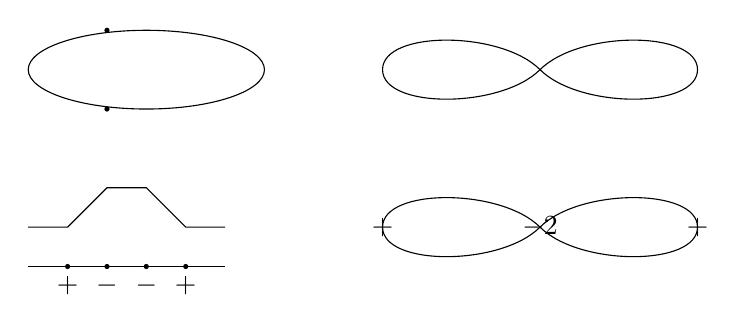
\begin{tikzpicture}


            \draw  (-2.5,0.5) ellipse (1.5 and 0.5);
            \draw (2.5,0.5) .. controls (2,0) and (0.5,0) .. (0.5,0.5) .. controls (0.5,1) and (2,1) .. (2.5,0.5) .. controls (3,0) and (4.5,0) .. (4.5,0.5) .. controls (4.5,1) and (3,1) .. (2.5,0.5);
            \node[circle, scale=.2, fill] at (-3,1) {};
            \node[circle, scale=.2, fill] at (-3,0) {};
            \draw (-4,-2) -- (-1.5,-2);
            \draw (-4,-1.5) -- (-3.5,-1.5) -- (-3,-1) -- (-2.5,-1) -- (-2,-1.5) -- (-1.5,-1.5);
            \node[circle, scale=.2, fill] at (-3.5,-2) {};
            \node[circle, scale=.2, fill] at (-3,-2) {};
            \node[circle, scale=.2, fill] at (-2,-2) {};
            \node[circle, scale=.2, fill] at (-2.5,-2) {};
            
            
            \node[below] at (-3.5,-2) {$+$};
            \node[below] at (-3,-2) {$-$};
            \node[below] at (-2,-2) {$+$};
            \node[below] at (-2.5,-2) {$-$};
            
            \begin{scope}[shift={(0,-2)}]
            \draw (2.5,0.5) .. controls (2,0) and (0.5,0) .. (0.5,0.5) .. controls (0.5,1) and (2,1) .. (2.5,0.5) .. controls (3,0) and (4.5,0) .. (4.5,0.5) .. controls (4.5,1) and (3,1) .. (2.5,0.5);
            
            \end{scope}
            
            \node at (0.5,-1.5) {$+$};
            \node at (4.5,-1.5) {$+$};
            \node at (2.5,-1.5) {$-2$};
            \end{tikzpicture}


\end{remark}


%label:"art:BoundedRationalEquiavlenceInRrN"
%type:"article"
%name:"bounded rational equiavlence in $\RR^n$"
%caption:""
%parent:"art_TropicalChowGroupsII"


%label:"def:TropicallyNumericalEquivalenct"
%type:"definition"
%name:"tropically numerical equivalenct"
%caption:""
%parent:"art_BoundedRationalEquiavlenceInRrN"


    Let $Q\subset \RR^n$ be a cycle of codimension $k$. We obtain a map 
    \begin{align*}
        d_Q: Z_k(\RR^n)\to \ZZ\\
        P\mapsto \deg(P\cdot Y)
    \end{align*}


We say that $Q_1$ is numerically equivalent to $Q_2$ if $d_{Q_1}=d_{Q_2}$.
\end{definition}
Observe that if $Q_1\sim^b Q_2$, this is the same as saying that $Q_1-Q_2\sim^b 0$, which implies that $d_{Q_1}-d_{Q_2}=0$. It is natural to ask if the converse hold. We first understand the question locally, i.e. the intersection of fans. 
%label:"prp:DDeterminesAFan"
%type:"proposition"
%name:"d determines a fan"
%caption:""
%parent:"art_BoundedRationalEquiavlenceInRrN"


    If $Q_1, Q_2\subset \RR^n$ are fans in $\RR^n$, then $d_{Q_1}=d_{Q_2}$ tells us that $Q_1 = Q_2$. 


\begin{corollary}
    If $Q_1\sim^b Q_2$ are bounded equivalent fans, they are the same fan. 
\end{corollary}
The plan: 
\begin{enumerate}
    \item Associate to a cycle $Q$ a fan $Q'$,
    \item Show that $Q\sim^b Q'$, 
    \item use the previous results. 
\end{enumerate}

For the first part: Let $\sigma\subset \RR^n$ be the polyhedron. Define the recession cone 
\[\text{Rec}(\sigma):= \{v\in \RR^ \st q+\RR_{\geq 0} v \subset \sigma \forall q\in \sigma\}\]
For sufficiently fine polyhedral structure on $Q$, one can show that the $\text{Rec}(X):=\{\text{Rec}(\sigma), \sigma\in X\}$ comes with the structure of a balanced fan.  This essentially is just ``zooming out'' really far away from your variety. 
%label:"thm:CyclesAndRecessionCones"
%type:"theorem"
%name:"cycles and recession cones"
%caption:""
%parent:"art_BoundedRationalEquiavlenceInRrN"


    Let $Q\subset \RR^n$ be a cycle. It is bounded rationally equivallent to its recession cone, that it: $Q\sim^b \text{Rec}(Q)$


The main proof of the theorem is the following. 
%label:"prp:TropicalCyclesAsSums"
%type:"proposition"
%name:"tropical cycles as sums"
%caption:""
%parent:"art_BoundedRationalEquiavlenceInRrN"


    Any cycle $Q$ can be written as a sum, 
    \[Q=\sum(Q_i+\vec v_i)\]
    where each $Q_i$ is a fan. 


%label:"prf:TropicalCyclesAsSums"
%type:"proof"
%name:"tropical cycles as sums"
%caption:""
%parent:""


    Every $q\in Q$ has a neighborhood $\text{Star}_Q(p)$ which looks like a fan. For any fan $P$, we define its splitting dimension $\dim_s(P)$ to be the maximum $k$ so that 
    \[P=\sum P_i\]
    where the $P_i$ have at least $k$-dimensional translation invariance. We then define $\dim_s(q):= \dim_s(\text{Star}_Q(p)$. 
    The proof then proceeds by removing first the star fans of points with star fan dimension 0, and then proceeding through the tropical subvariety. 


We obtain the proof of the theorem:
\begin{align*}
    \text{Rec}(Q)=& \text{Rec}(\sum Q_i + \vec v_i) \\
    = &\sum \text{Rec}(Q_i + \vec v_i) = \sum Q_i \sim^b \sum Q_i+\vec v_i = Q
\end{align*}
In summary, the following are equivalent:
\begin{align*}
    Q_1\sim^b Q_2 && d_{Q_1} = d_{Q_2} && \text{Rec}(Q_1)= \text{Rec}(Q_2)


\end{align*}
